\chapter{Multiobject tracking using deep learning and tracking by detection}
In this chapter, the solution developed for solving the multiobject visual tracking problem using deep learning and tracking-by-detection is explained.

\section{Design}
The main contribution of this work is the development of a visual tracking algorithm capable of tracking different types of objects using deep learning techniques. To achieve this task the selected tracking methodology is the tracking by detection. Our method combines detections coming from an object detection neural network with classic visual tracking techniques. With this combination, the final system provides a balance between speed and accuracy. The detections from the neural networks are usually slower than a pure tracking but more accurate and robust whereas the tracker results are often quick but slightly more inaccurate.\\
A software application, named \textit{dl-objecttracker}, has been designed and developed which implements the proposed multiobject visual tracking algorithm. The module architecture of this application is summarized in the diagram of Figure \ref{fig:general}.
\begin{figure}[H]
\begin{center}
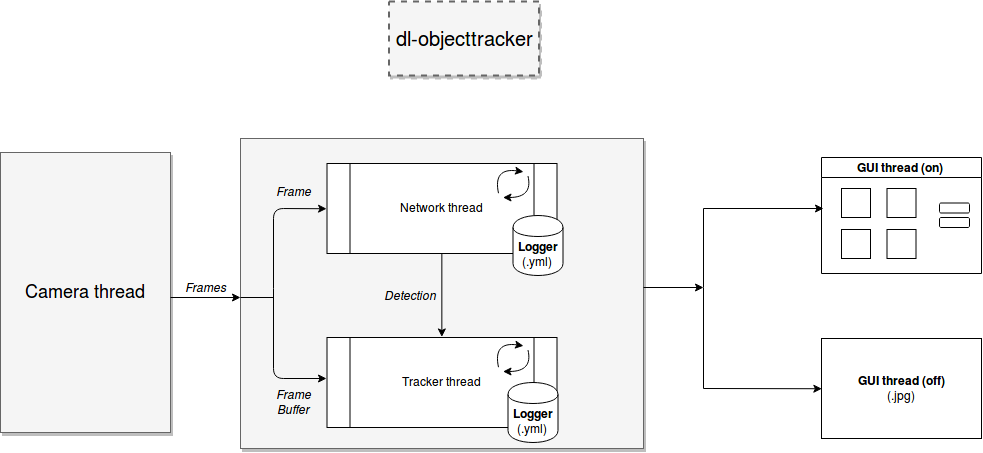
\includegraphics[scale=0.4]{figures/general.png}
\caption{Modular architecture of the dl-objecttracker application}
\label{fig:general}
\end{center}
\end{figure}

As it can be seen the system is built in a modularized way with different threads. There are four threads: Camera, GUI, Network and Tracker. All of them are going to be discussed more in depth on its corresponding sections of this chapter but the general workflow of the system is going to be explained here (Figure \ref{fig:update_cam}).\\
First, the camera thread provides the images or frames to the rest of the threads, i.e.\ it is in charge of the input to the system. The output of the system can be provided using a mechanism of \textit{logging} of the results per frame or using the GUI. If the GUI is configured to show the graphical interface (\textit{on}), the results are shown on the screen. But if the graphical interface is not configured (\textit{off}) the results are saved in JPG files.\\ The core of the computing is divided into the Network thread and the Tracker thread. This Tracker has a buffer of frames of different size coming from the Camera to work on \textit{delayed real-time}. So, when the first frame is available it is given to the Network thread which starts doing the inference, i.e.\, it starts detecting objects. Meanwhile, the buffer is accumulating the incoming frames from the Camera until the detection from the Network comes.\\
When the neural detection is available, the Tracker thread starts the tracking of the detected objects inside the buffer of frames. The last frame in the buffer is used to feed again the Network allowing for a synchronism between the neural detections and the tracking in the frames. This timing can be observed more clearly in the Figure \ref{fig:buffer}.
\begin{figure}[H]
\begin{center}
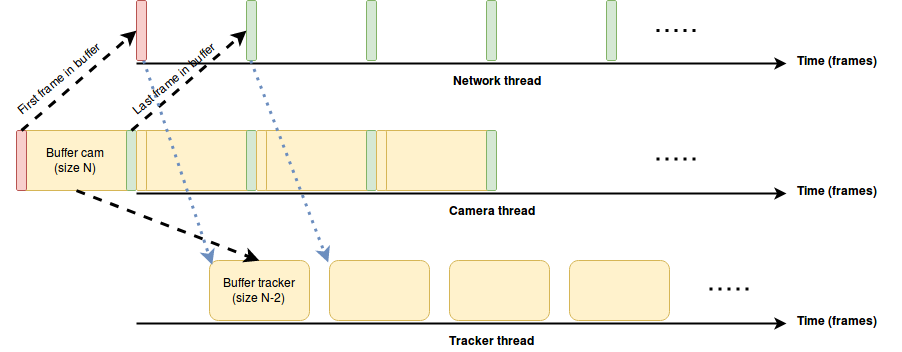
\includegraphics[scale=0.4]{figures/buffer.png}
\caption{How the buffer is handled}
\label{fig:buffer}
\end{center}
\end{figure}
It can be seen that given a complete buffer in Camera of size \textit{N}, the first frame is assigned to the Network and, when this frame is processed, a buffer of size \textit{N-2} is assigned to the Tracker to be processed. The last frame of the given buffer is passed to the Network again. This iterative mechanism continues in time ensuring that no frame is lost or ignored while the neural processing takes place at its own pace, which can be much slower than the input frame rate. After the first iteration, the length of the size passed to the Tracker is \textit{N-1}. The application has always a delay in output frames of 1 buffer (\textit{delayed real-time}).
\\As commented before, the buffer changes its size in every iteration but we can not allow the buffer to increase or decrease this size in an uncontrolled way because that will end blocking the application. If the buffer is too big, the tracking will take more time and the neural network will finish before the tracking is done. This is, the Network is underused. In the other side, if the buffer is too small the Tracker will end its work before the inference is done in the Network so the Tracker will have to wait much more time to the Network to finish (Tracker underused). For these reasons a balance is needed.\\
The neural network inference time is approximately always the same so this time is taken as reference. Then, the only part of this processing core where we can change is on the Tracker side. The obtained solution consists of a Tracker which constantly measures its frame rate (FPS) allowing it to slow down or speed up depending on the Tracker processing speed.\\
Once all the frames have been processed the Network and Tracker thread stop. After that, the results are logged into the YML files (a file for each frame) and the user can close the application.\\
The general behavior of the application when running video sequences or raw frames was presented. Nevertheless, it can also handle live stream videos coming from local cameras connected. In this case, the logging of the results is not performed but the tracking by detection scheme is the same.\\
The ``main" is done in the \texttt{update} function of the Camera which is continuously called by the Camera thread. As the system architecture is based in multiple threads, the synchronism between them is crucial. Because of this, the control of the application is done taking into account the synchronism between all the threads, their internal status and variables.
\begin{figure}[H]
\begin{center}
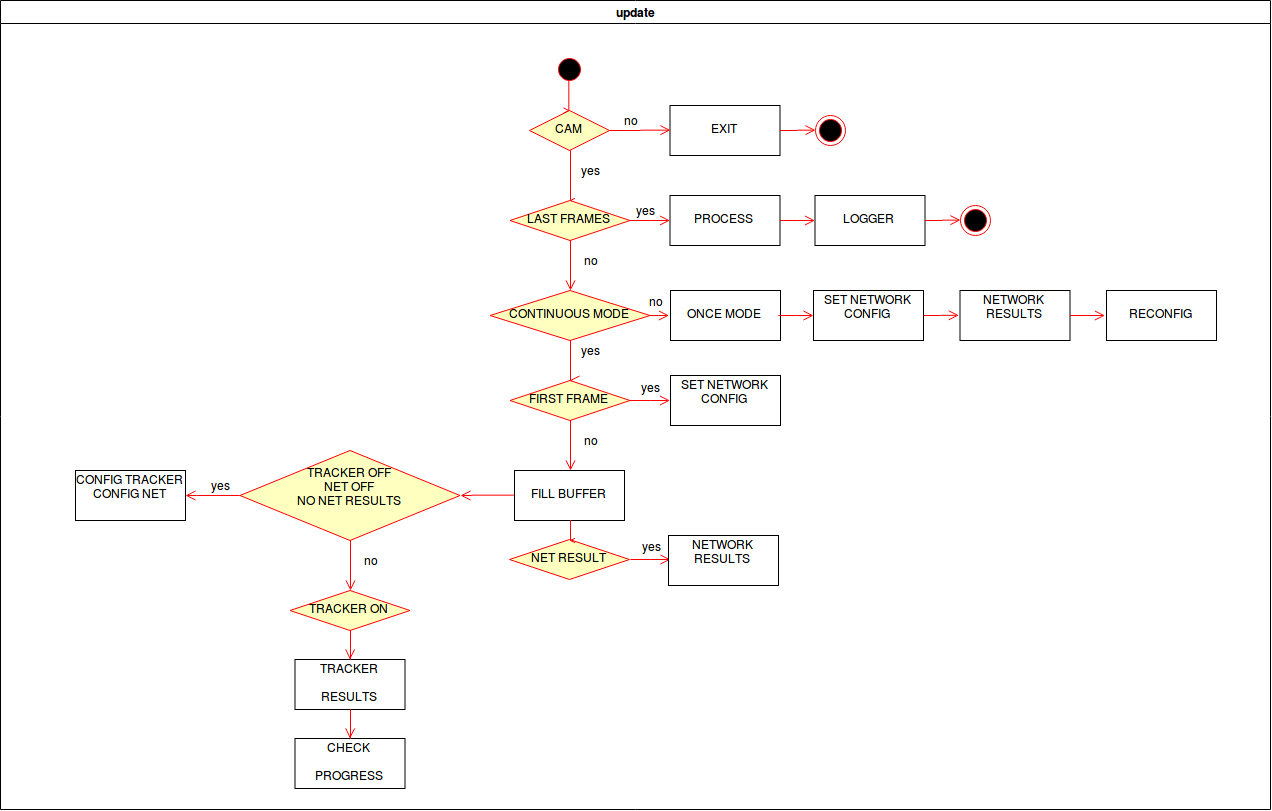
\includegraphics[scale=0.33]{figures/update_camera.png}
\caption{The control flow}
\label{fig:update_cam}
\end{center}
\end{figure} 

The application is configurable using an YML file (\textit{objecttracker.yml}). For the instructions on how to run the application please refer to the wiki of the project (see \ref{Methodology}).
\\In the next sections the implementation of each thread of the system is explained, including the available configuration modifications.\\

\section{Video source module}
The Camera module provides the input images to the rest of the system. These images can be obtained using four different sources:
\begin{itemize}
    \item \textbf{Local camera (with OpenCV)}: the Camera can read from a local camera using the OpenCV routine \texttt{VideoCapture} indicating the device number of the camera.
    \item \textbf{Local camera (with ROS)}: the Camera can use ROS to read from the camera device. In order to do so, the user needs to launch a terminal and type \texttt{roslaunch usb\_cam.launch}. This will publish a ROS topic \texttt{/usb\_cam/image\_raw} that can be subscribed by the Camera module and it will start reading frames from the device. For more information about the launching process please refer to the wiki of the project\footnote{\href{https://jderobot.org/Arodriguez-tfm\#Week_24:_Introducing_ROS}{Wiki: ROS}}.
    \item \textbf{Local video}: to read from a local video the OpenCV routine \texttt{VideoCapture} is also used but indicating the video path in the configuration file.
\item \textbf{Local image files}: the path containing all the image files is required to be passed to \texttt{VideoCapture}. This video source is very useful because most of the datasets are provided as sequences of frames instead of videos. And it can avoid problems such as creating sequences of videos with the wrong duration or frame rate.
\end{itemize}
The Camera thread source and options can be modified at the configuration file. The source is selected at \texttt{ObjectTracker->Source}. After that the user is required to indicate the device number \texttt{ObjectTracker->Local->DeviceNo} if using a local camera with OpenCV, the video path \texttt{ObjectTracker->Video->Path} if using a local video or the images path \texttt{ObjectTracker->Images->Path} when using local image files.\\
The user needs to modify the \texttt{usb\_cam.launch} to change the Camera configuration when using ROS.\\
Before being sent to other threads the image is rescaled according to the neural network input size. It continues all the process with this standard size. When the final results are obtained this scaling is taken into account to rescale again the coordinates of the detections or trackers with respect to the original image size.\\
Apart from providing images the Camera thread also controls the flow of the application. It has been implemented in this way because the application offers the option of not having GUI. In the first versions of the project the control of the application (the ``main") was implemented in the GUI thread but when the no-GUI option was added this was moved to the Camera thread.\\

\section{GUI module}
The GUI module provides the interface with the human user and, as commented before, is optional. It was implemented using the tools provided by PyQt5, in particular with the packages \textit{QtGui, QtCore} and \textit{QtWidgets}.\\
The graphical interface has four windows and two buttons. The top-left window shows the input frames in real-time while the top-right one shows the final results. The intermediate results obtained from the Network and the Tracker will be provided at the bottom part of the display. The application with GUI has two modes with its respective buttons: ``run continuous" and ``run now". In the first one, the application runs continuously until it finishes the processing (the program finishes depending on the image source). In the second one, the user can push the \textit{Run now} button to make a single Network detection on the current frame and to continue the tracking from that frame onward.
\begin{figure}[H]
\begin{center}
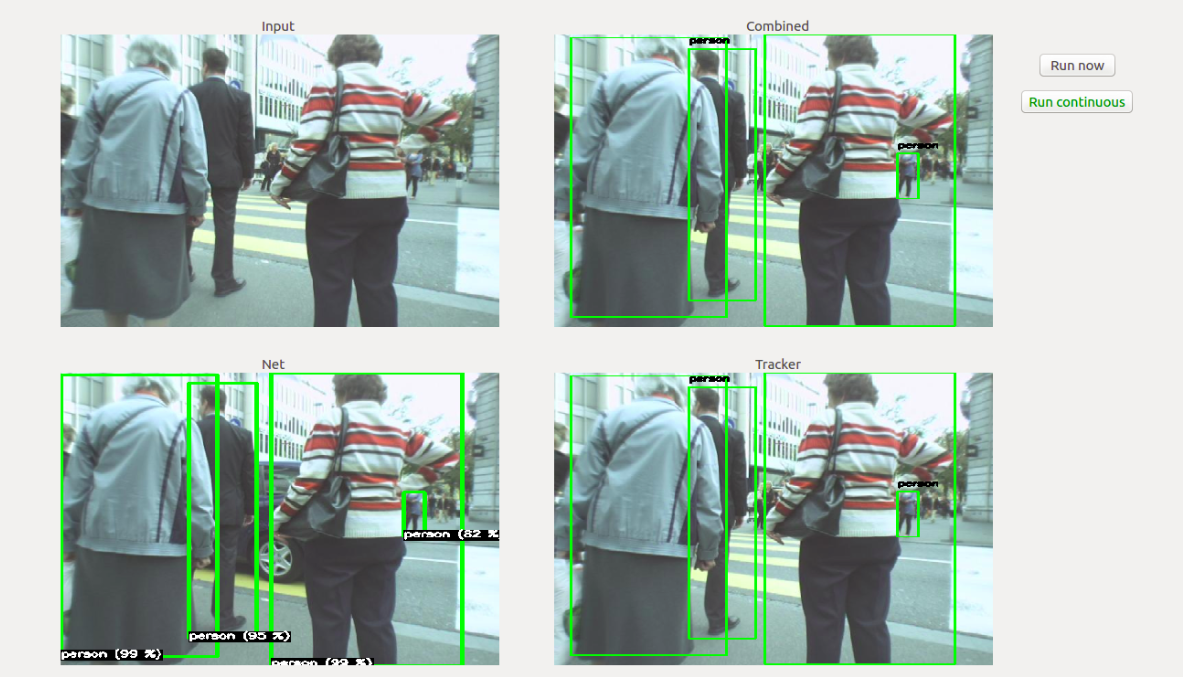
\includegraphics[scale=0.35]{figures/gui.png}
\caption{The graphical user interface of the dl-objecttracker application}
\label{fig:gui}
\end{center}
\end{figure} 
\section{Neural Network module}\label{neural_networks}
The Network module is tasked with the object detections in the images, which feed the Tracker on every iteration. It supports Tensorflow and Keras object detection models. The Tensorflow models can be obtained from the Tensorflow detection model zoo\footnote{\href {https://github.com/tensorflow/models/blob/master/research/object_detection/g3doc/detection_model_zoo.md}{Tensorflow detection model zoo}} and include SSD and R-CNN detectors. The Keras models are limited to SSD architectures and it can be obtained from this set\footnote{\href {https://github.com/pierluigiferrari/ssd_keras#download-the-original-trained-model-weights}{Keras models}}.\\
The datasets on which the model was trained need to be specified to assign the labels to the objects. The supported labels include the VOC, COCO, KITTI, OID and PET datasets.\\ As it ocurred with the Camera module, the Network module has configurable options available in \textit{objecttracker.yml}:
\begin{itemize}
    \item \texttt{Framework}: Keras or Tensorflow
    \item \texttt{Model}: the model file
    \item \texttt{Dataset}: VOC/COCO/KITTI/OID/PET
    \item \texttt{Input size}: this input size can be modified depending on the selected model. Some models do not allow to change the input image size
    \item \texttt{Confidence}: the confidence threshold for the detections obtained. If a detection obtains a confidence value below that detection is discarded
\end{itemize}
The Network thread basically receives an image (previously resized) and performs the inference. As a result it outputs the detections obtained in the image (if any) and it draws these detections in form of bounding boxes containing also the label and the confidence value.\\
The logging of the Network and Tracker results are optional and it can be changed at the YML configuration file in \texttt{ObjectTracker->Logger->Status}. These results are logged in the \texttt{logNetwork} and \texttt{logTracker} functions respectively.\\

\subsection{Tensorflow models} \label{tf_models}
These models are obtained from the Tensorflow detection model zoo which provides models for inference out-of-the-box, i.e.\ to be directly used. Among the available models only some of them were tested for its use in the project. The pre-trained models used were trained on the COCO dataset because the available classes in this dataset were considered enough for the type of objects that can be seen in the tracking sequences used.\\ In the table \ref{tab:tf_models}, the Tensorflow models performance can be seen:
\begin{table}[H]
\begin{center}
\begin{tabular}{|c|c|c|}
\hline
Model name                                 & Speed (FPS) & COCO mAP \\ \hline
\textbf{ssd\_mobilenet\_v2\_coco}          & 32         & 22       \\ \hline
\textbf{faster\_rcnn\_inception\_v2\_coco} & 17         & 28       \\ \hline
\textbf{mask\_rcnn\_inception\_v2\_coco}   & 13         & 25       \\ \hline
\end{tabular}
\end{center}
\caption{Tensorflow models performance (from \href{https://github.com/tensorflow/models/blob/master/research/object_detection/g3doc/detection_model_zoo.md#coco-trained-models}{Tensorflow detection model zoo})}
\label{tab:tf_models}
\end{table}
The COCO mAP numbers here are evaluated on COCO 14 minival set using the \href{http://cocodataset.org/#detection-eval}{MSCOCO evaluation protocol}. The reported running time in ms is measured for 600x600 images (including all pre and post-processing). The AP scores are averaged over multiple Intersection over Union (IoU) values as the MSCOCO evaluation protocol indicates. As the authors say, ``these timings depend highly on one's specific hardware configuration (performed using an Nvidia GeForce GTX TITAN X card) and should be treated more as relative timings in many cases". However, some characteristics of each model can be extracted in terms of speed and accuracy. As expected, the R-CNN models achieve better accuracy while performing a little slower with respect to SSD.

\subsubsection{SSD MobileNetV2}
This SSD implementation uses MobileNetV2 as backbone. As commented in section \ref{mobilenet}, MobileNetV2 is a network proposed to work on mobile devices, this can be interesting to the project because of the hardware limits (it needs to work on CPU only).
\subsubsection{Faster R-CNN InceptionV2}
This region-based model was discussed in section \ref{mobilenet}. The implementation uses InceptionV2 \cite{szegedy2016rethinking} as the feature extractor. This backbone follows the idea of its predecesor (InceptionV1) and adds two main ideas: reduce the representational bottleneck and use smart factorization methods. Refering to the first one, the intuition is that neural networks usually perform better when the convolutions do not alter the dimensions of the input in a drastical way (may cause loss of information). To solve this problem they expand the inception module making it wider (instead of deeper). Apart from that, the convolutions are made more efficient in terms of computational complexity. The authors propose factorizing the 5x5 convolution into two 3x3 convolution operations making it 2,78 times faster, among other improvements.
\subsubsection{Mask R-CNN InceptionV2}
This state-of-the-art instance segmentation network is used as object detection network because it offers the bounding boxes locations, apart from the instance masks (Figure \ref{fig:maskrcnn_tests}). The selected implementation also makes use of InceptionV2 as backbone.
\begin{figure}[H]
\begin{center}
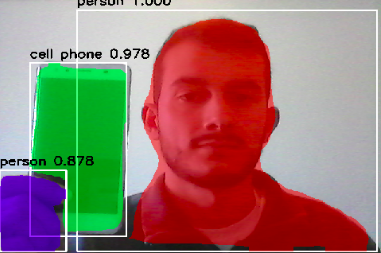
\includegraphics[scale=0.5]{figures/maskrcnn_first_tests.png}
\caption{First tests with Mask R-CNN using live video}
\label{fig:maskrcnn_tests}
\end{center}
\end{figure} 
\subsection{Keras models} \label{keras_models}
The Keras network is a Keras port of the SSD model architecture introduced by Wei Liu et al. in \cite{liu2016ssd} from SSD-Keras\footnote{\href{https://github.com/pierluigiferrari/ssd_keras}{SSD-Keras}}. The repository offers pre-trained models and allows the model training from scratch. The base network architecture used is VGG (see section \ref{mobilenet}). The pre-trained models used were trained on the PASCAL VOC dataset. The pre-trained models available included COCO and ILSVRC datasets but PASCAL was selected because COCO dataset was already used in the previous SSD model in Tensorflow. In the next table, it can be seen the author reported performance \cite{ssdkerasperf}:
\begin{table}[H]
\begin{center}
\begin{tabular}{|c|c|c|}
\hline
Model name               & Speed (FPS) & VOC2007 test mAP @ 0,5 \\ \hline
\textbf{SSD300\_VOC0712} & 39          & 77,5                   \\ \hline
\textbf{SSD512\_VOC0712} & 20          & 79,8                   \\ \hline
\end{tabular}
\end{center}
\caption{Keras models performance. Evaluated in the official Pascal VOC 2012 test server using an NVIDIA GeForce GTX 1070 mobile.}
\end{table}
The authors claim that their implementation performs slightly better than the original SSD implementation in Caffe\footnote{\href{https://github.com/weiliu89/caffe/tree/ssd}{SSD-Caffe}}.

\section{Tracker module}\label{tracker_algorithms}
The Tracker module is the core of the project and therefore it is going to be explained more in depth. As previously commented, the Tracker receives an input detection coming from the Network module and performs the multiobject visual tracking over a frame buffer of variable size following a tracking by detection scheme. This hybrid tracker it is intended to show the advantages of the tracking by detection with deep learning over a pure neural network tracking or a pure classic feature tracking.\\
The tracker can work in three operating regimes: \textit{slow, normal} and \textit{fast}. The calculation of this regime is performed using an internal buffer of FPS rates of size 3. The length selected is due to the fact that the tracker is required to respond quickly to changes in its velocity avoiding slowing down or speeding up in an excessive way. The tracker speed calculation is explained in Algorithm \ref{tracker_speed}. Three frame rate thresholds are established to distinguish between a tracker which is behaving in a ``normal way" or a slower or a faster processing time.\\ If the tracker is performing slower than normal the next three frames that are to be tracked are discarded from the buffer in the \texttt{imageToTrack} function. In the other hand, if the tracker is going too fast it is slowed down in \texttt{getOutputImage} by waiting some frames to return the image to be output.\\ With this mechanism the buffer does not increase or decrease too much in size allowing a more stable behavior and a good synchronization between the threads. This dynamic calculation allows the tracking to behave differently depending on the operating regime in which it is on each instant. However, it will be seen in the next chapter that this regime is very dependent on the tracker that is being used and its own performance.\\
\begin{algorithmic}[H]
\begin{algorithm}
\State \textbf{Inputs:} averageFPS, lastFPSBuffer, trackerSlow, trackerFast, counterSlow, counterFast
\State \textbf{Output:} trackerSpeedMode
\Procedure{trackerSpeedMode}{}
\If {not 0 in $lastFPSBuffer$ and $averageFPS$ \textless 10}
    \State $counterSlow$ + 1
    \If {$counterSlow$ == 3}
        \State $counterSlow$ = 0
        \State $trackerSlow$ = True
    \EndIf
\ElsIf{not 0 in $lastFPSBuffer$ and 10 \textless $averageFPS$ \textless 25}
    \State $trackerSlow$ = False
    \State $trackerFast$ = False
\ElsIf{$averageFPS$ \textgreater 25 and $counterFast$ \textless 1}
    \State $counterFast$ + 1
\State $trackerFast$ = True
\EndIf  
\EndProcedure
\caption{Tracker speed mode}\label{tracker_speed}
\end{algorithm}
\end{algorithmic}

\subsection{Confidence in tracking}\label{conf_in_tracking}
To check if the obtained tracking is acceptable or not the confidence value is used. The two libraries available to perform the tracking offer this feature so it is used with small differences. OpenCV returns a boolean value to show the confidence in the tracking, and that is directly used to threshold the tracking results. In the case of dlib, it returns a numerical value. The dlib threshold value was established to 7 based on examples of other works and some experiments.\\

\subsection{OpenCV trackers}
The tracking will be performed using several already built tracking implementations of two libraries: OpenCV and dlib. This will also allow for a good comparative between them that can lead us to select the preferred option for the tracking algorithm.\\
OpenCV is known for the great variety of algorithms for which it provides implemented solutions, one of them is tracking. Tracking libraries are included in the OpenCV extra modules (\texttt{opencv contrib}).\\
The tested OpenCV trackers include \textit{BOOSTING, MIL, MEDIANFLOW, TLD, KCF, MOSSE} and \textit{CSRT} (in release order). They are now introduced:
\begin{itemize}
\item BOOSTING \cite{grabner2006real}: based on an online version of AdaBoost, the tracker is trained at runtime with positive and negative examples of the object to track. An initial bounding box needs to be provided by the user or other object detection algorithm. The classifier looks over the pixel neighborhood of a previous location to find the new location. The classifier is constantly updated with these new positives.
\item MIL \cite{babenko2009visual}: the \textit{Multiple Instance Learning} algorithm tries to solve the problem of learning an adaptive appearance model for object tracking. To achieve this, the authors train a discriminative classifier online to separate the object to track from the background, i.e.\ positive and negative examples are extracted from the frame (Figure \ref{fig:mil}). Similarly to the Boosting algorithm, the model searches inside of the window of the old location. It obtains a probability map with most probably new location of the object and updates the tracker model.
\begin{figure}[H]
\begin{center}
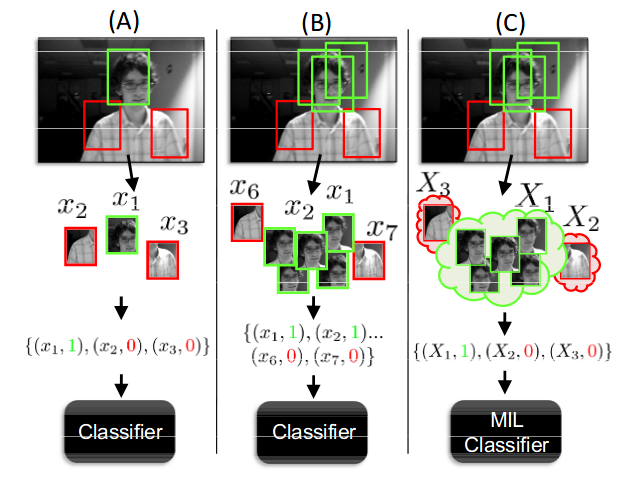
\includegraphics[scale=0.5]{figures/mil.png}
\caption{Updating a discriminative appearance model: (A) using a single positive image patch. (B) using several positive image patches. (C) using one positive bag of several image patches (from \cite{babenko2009visual})}
\label{fig:mil}
\end{center}
\end{figure}
\item MEDIANFLOW \cite{kalal2010forward}: the Median Flow algorithm introduced a novel method for tracking failure detection based on the Forward-Backward error. This  basically consists of performing the tracking forward and backward in time in a given frame and measure the discrepances between trajectories (see Figure \ref{fig:medianflow}). The authors claim that these discrepances are highly correlated with real tracking failures.
\begin{figure}[H]
\begin{center}
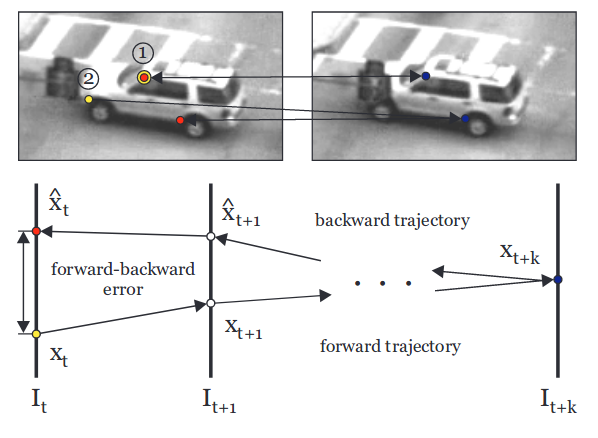
\includegraphics[scale=0.4]{figures/medianflow.png}
\caption{The forward-backward error in Point 2 (from \cite{kalal2010forward})}
\label{fig:medianflow}
\end{center}
\end{figure}    
\item TLD \cite{kalal2011tracking}: in the original paper on which is based the implementation, the authors investigate the long-term object tracking and propose a novel framework that descomposes this type of tracking into \textit{tracking, learning and detection} (TLD). The tracker based on Median Flow follows the object in every frame. The detector is composed by a patch variance module, followed by an ensemble classifier and finally a Nearest Neighbor classifier. The function of this detector is to correct the tracker if necessary. The learning step estimates the errors of the detector and updates it using a novel method called \textit{P-N learning}.
\item KCF \cite{henriques2012exploiting}: the \textit{Kernelized Correlation Filter} is a tracking framework that utilizes properties of circulant matrix to enhance the processing speed. The authors observed that the translated and scaled patches used to train discriminative classifiers contain redundancies and the resulting data matrix from these patches is circulant. With kernel regression as classification method they derive the KCF tracking.
\item MOSSE \cite{bolme2010visual}: correlation filters can track complex objects in common tracking scenarios that may include rotations, occlusions or other distractions at high frame rates. The \textit{Minimum Output Sum of Squared Error} filter is another type of correlation filter. Filter based trackers model the appearance of objects using filters trained in example images (Figure \ref{fig:mosse}). With a given initial target in the first frame the tracking and the filter training start to work together. The idea behind MOSSE is an optimization problem, given a set of training images $f_i$ and training outputs $g_i$, MOSSE finds a filter \textit{H} that minimizes the sum of squared error between the actual output of the convolution and the desired output of the convolution (see Formula \ref{eq:conv_mosse}).
\begin{equation}
\min_{H^*}\sum_{i}\left|F_i \odot H^* - G_i\right|^2
\label{eq:conv_mosse}
\end{equation}

\begin{figure}[H]
\begin{center}
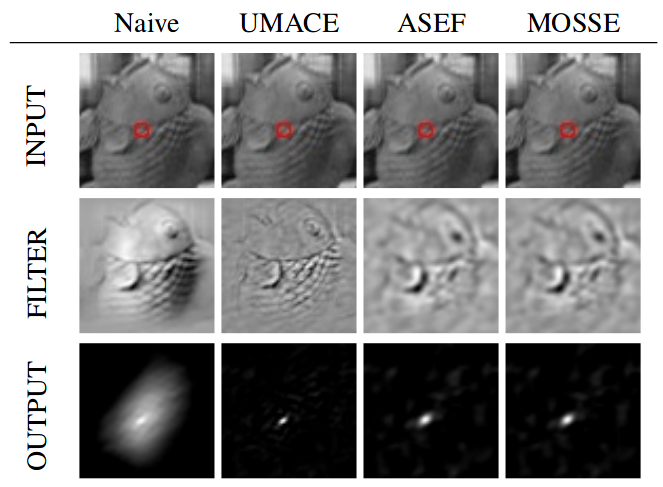
\includegraphics[scale=0.35]{figures/mosse_filter.png}
\caption{Comparison of the output peaks produced by different correlation filters (from \cite{bolme2010visual})}
\label{fig:mosse}
\end{center}
\end{figure} 

\item CSRT \cite{lukezic2017discriminative}: the CSRT tracker is based on the paper \textit{Discriminative Correlation Filter with Channel and Spatial Reliability}. Here the authors introduce the channel and spatial reliability concepts to DCF tracking to improve the filter update and the tracking process (Figure \ref{fig:csrt}). The spatial information is used to restrict the searching to the parts suitable for tracking. In the other hand, the channel information aims to reduce the noise of the weighted-averaged filter response.
\begin{figure}[H]
\begin{center}
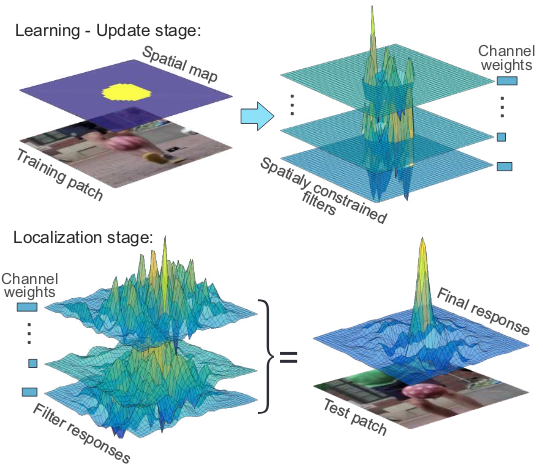
\includegraphics[scale=0.4]{figures/csrt.png}
\caption{Overview of the CSR-DCF approach (from \cite{lukezic2017discriminative})}
\label{fig:csrt}
\end{center}
\end{figure} 
\end{itemize}

In the next chapter, some experiments are performed to put into practice the advantages and disadvantages of each OpenCV tracker. Furthermore, the dlib tracking will also be discussed allowing for a comparison between all the proposals and allowing us to select the best tracker option.
\subsection{dlib trackers}
In chapter 2 the \texttt{dlib} library was introduced as a set of independent software components that provide different utilities, one of them is tracking. The \texttt{dlib.correlation\_tracker} is going to be used for this project. As its name indicates, it is another implementation of a correlation filter for tracking which has been widely used. This tool is an implementation of the method described in \cite{danelljan2014accurate}.\\ In the proposed solution, the authors are centered in solving the challenging problem of handling large scale variations in visual object tracking. They propose a method for a robust scale estimation in a tracking by detection framework, as it is the case in this project. To do so the learning of discriminative correlation filters is based on a scale pyramid representation.
